\section{Adaptive-mesh refinement and DG}
With the Discontinuous Galerkin method, using AMR brings additional complexity into the evaluation of face integrals described in \Cref{Final_Integration_Fn_b}, \Cref{singleNumIntBface}.
To describe the process in detail, definition of the numerical flux \Cref{NumFluxDef} needs to be taken into account. What is evaluated during the assembling procedure \Cref{algorithm:singleTimeStep} is the term \Cref{singleNumIntBface}. In order to evaluate it, we need to consider values of the solution in quadrature points $\left\{\bfx^{ij}_1, ..., \bfx^{ij}_{\bfn_f}\right\}$ from both sides of $\Gamma_{ij}\in \Gamma_I$, that is from the two neighboring elements $K^i\in T, K^j\in T$. For $\Gamma_{ij}\in \Gamma_B$ the situation is obviously simpler as is not discussed further.
\paragraph{}
What needs to be evaluated is in fact the term
\be
\mrH\lo{\mrPsi_h^{k}}|_{ij}\lo\bfx\ro, {\mrPsi_h^{k}}|_{ji}\lo\bfx\ro, \bfn_{ij}\lo\bfx\ro\ro
\ee
If the two neighboring elements are of the same size as in \Cref{figure:simpleNeighbors}, calculation of this term from algorithmic perspective is performed as follows:\\
\begin{algorithm}[H]
\KwData{$K^i\in T_h$}
\KwData{$\Gamma_{ij}\in \Gamma_I\ $ a face of $K^i$}
\KwData{Quadrature points $\left\{\bfx^{ij}_1, ..., \bfx^{ij}_{\bfn_f}\right\}$}
\# \textbf{1}. Triangulation and DOFs handling\\
Find the neighbor $K^j$ (querying data structures representing the mesh $T$)\\
Find the set of degrees of freedom (basis functions) $v_h^i = v_h \lo K^i\ro$\\
Find the set of degrees of freedom (basis functions) $v_h^j = v_h \lo K^j\ro$\\

\# Loop over quadrature points\\
\ForEach{$\bfj_f \in \left\{1, ..., \bfn_f\right\}$}
{
	\# \textbf{2}. Previous solution values\\
	Find previous solution value $\bfw_{\bfj_f}^{ip} = {\mrPsi_h^{k}}|_{ij}\lo\bfx_{\bfj_f}\ro$ on $K^i$\\
	Find previous solution value $\bfw_{\bfj_f}^{jp} = {\mrPsi_h^{k}}|_{ij}\lo\bfx_{\bfj_f}\ro$ on $K^i$\\
	Set: $\bfn_{\bfj_f} = \bfn_{ij}\lo\bfx_{\bfj_f}\ro$\\
	\# \textbf{3}. Numerical flux evaluation\\
	$\mrH\lo{\mrPsi_h^{k}}|_{ij}\lo\bfx\ro, {\mrPsi_h^{k}}|_{ji}\lo\bfx\ro, \bfn_{ij}\lo\bfx\ro\ro
		= \mrH\lo\bfw_{\bfj_f}^{ip}, \bfw_{\bfj_f}^{jp}, \bfn_{\bfj_f}\ro$\\
		
	\# ... (Further processing as in \Cref{algorithm:singleTimeStep})
}
\ \\
\caption{Assembling of numerical flux}
\label{algorithm:numFluxSimple}
\end{algorithm}

\begin{figure}[H]
		\begin{center}
			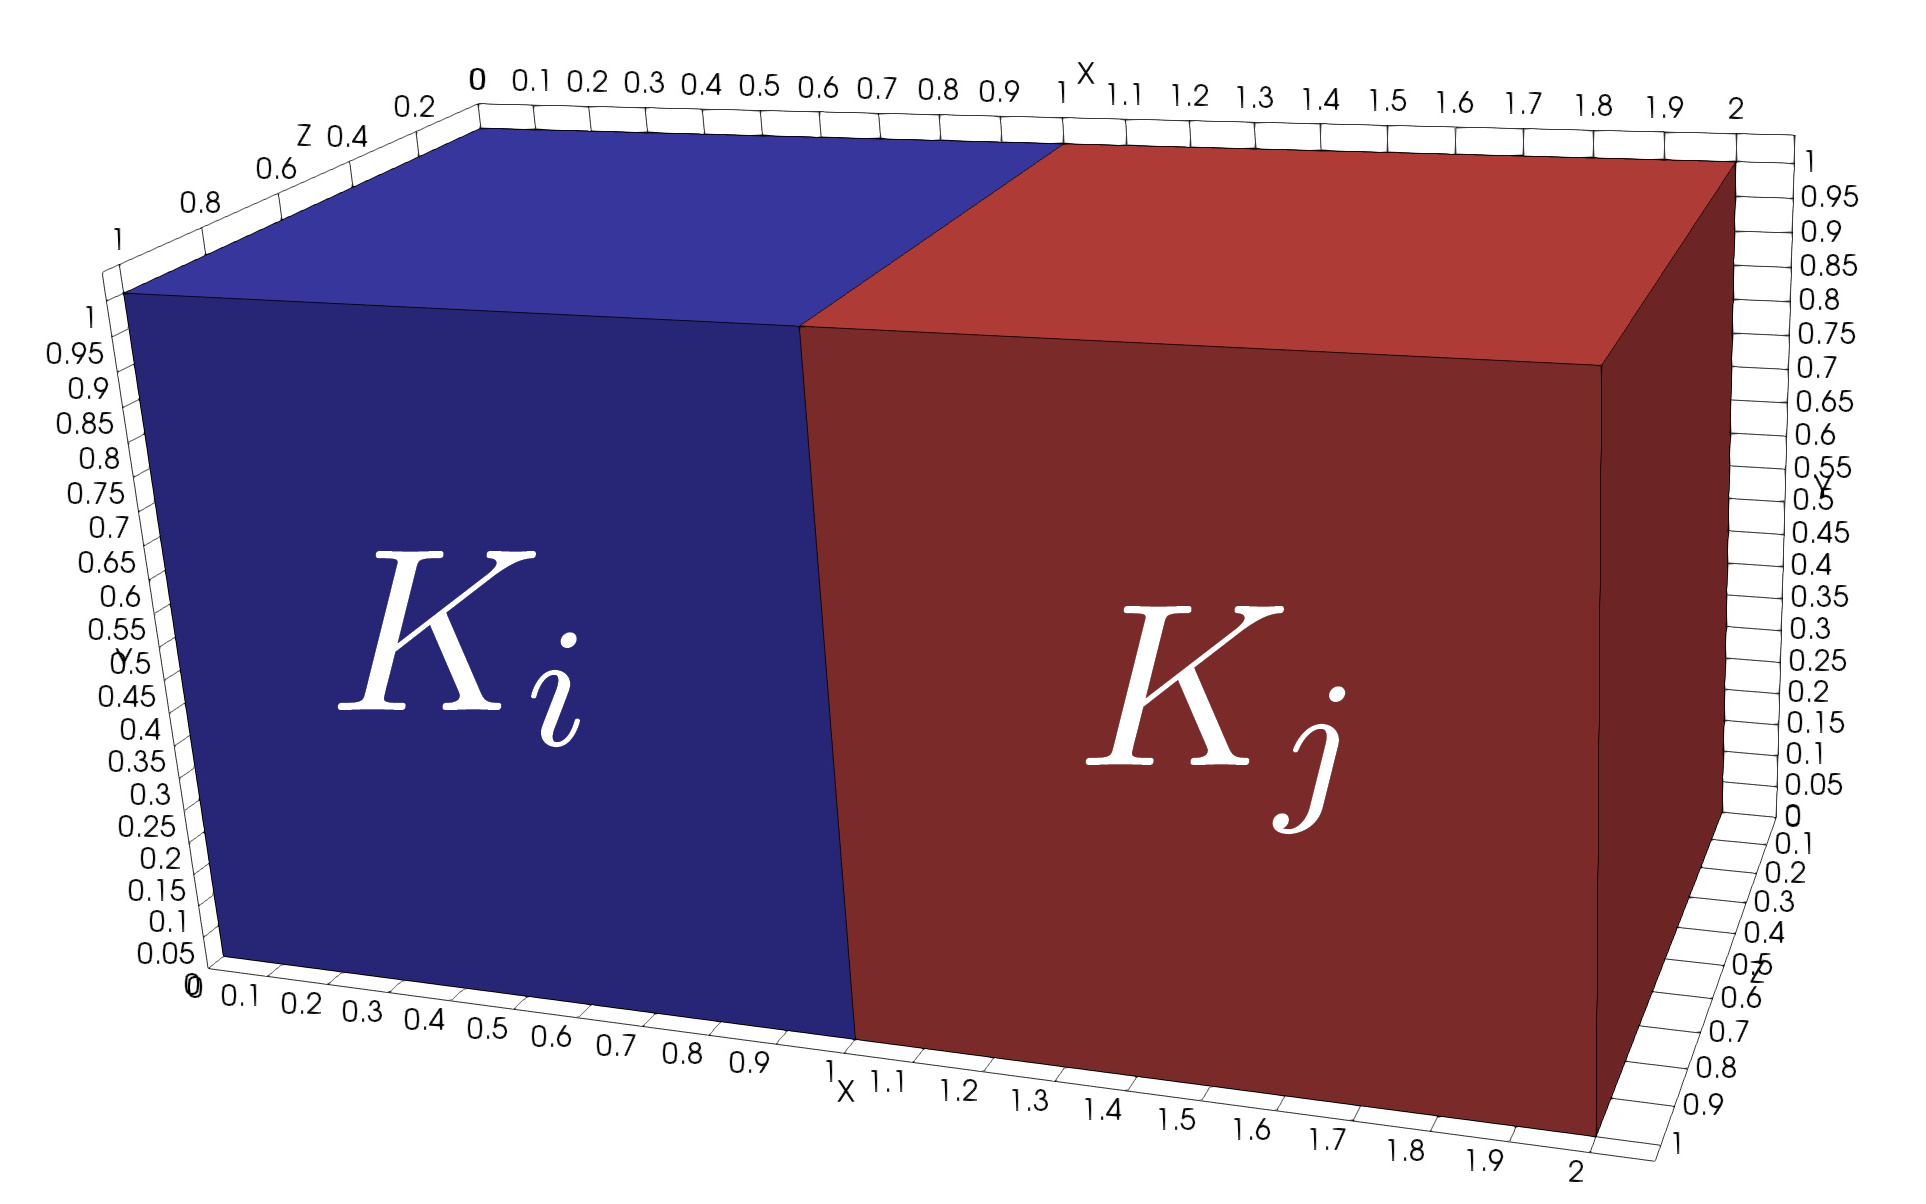
\includegraphics[width=0.5\textwidth]{img/mesh/neighborsK.jpg}
			\vspace{3mm}
			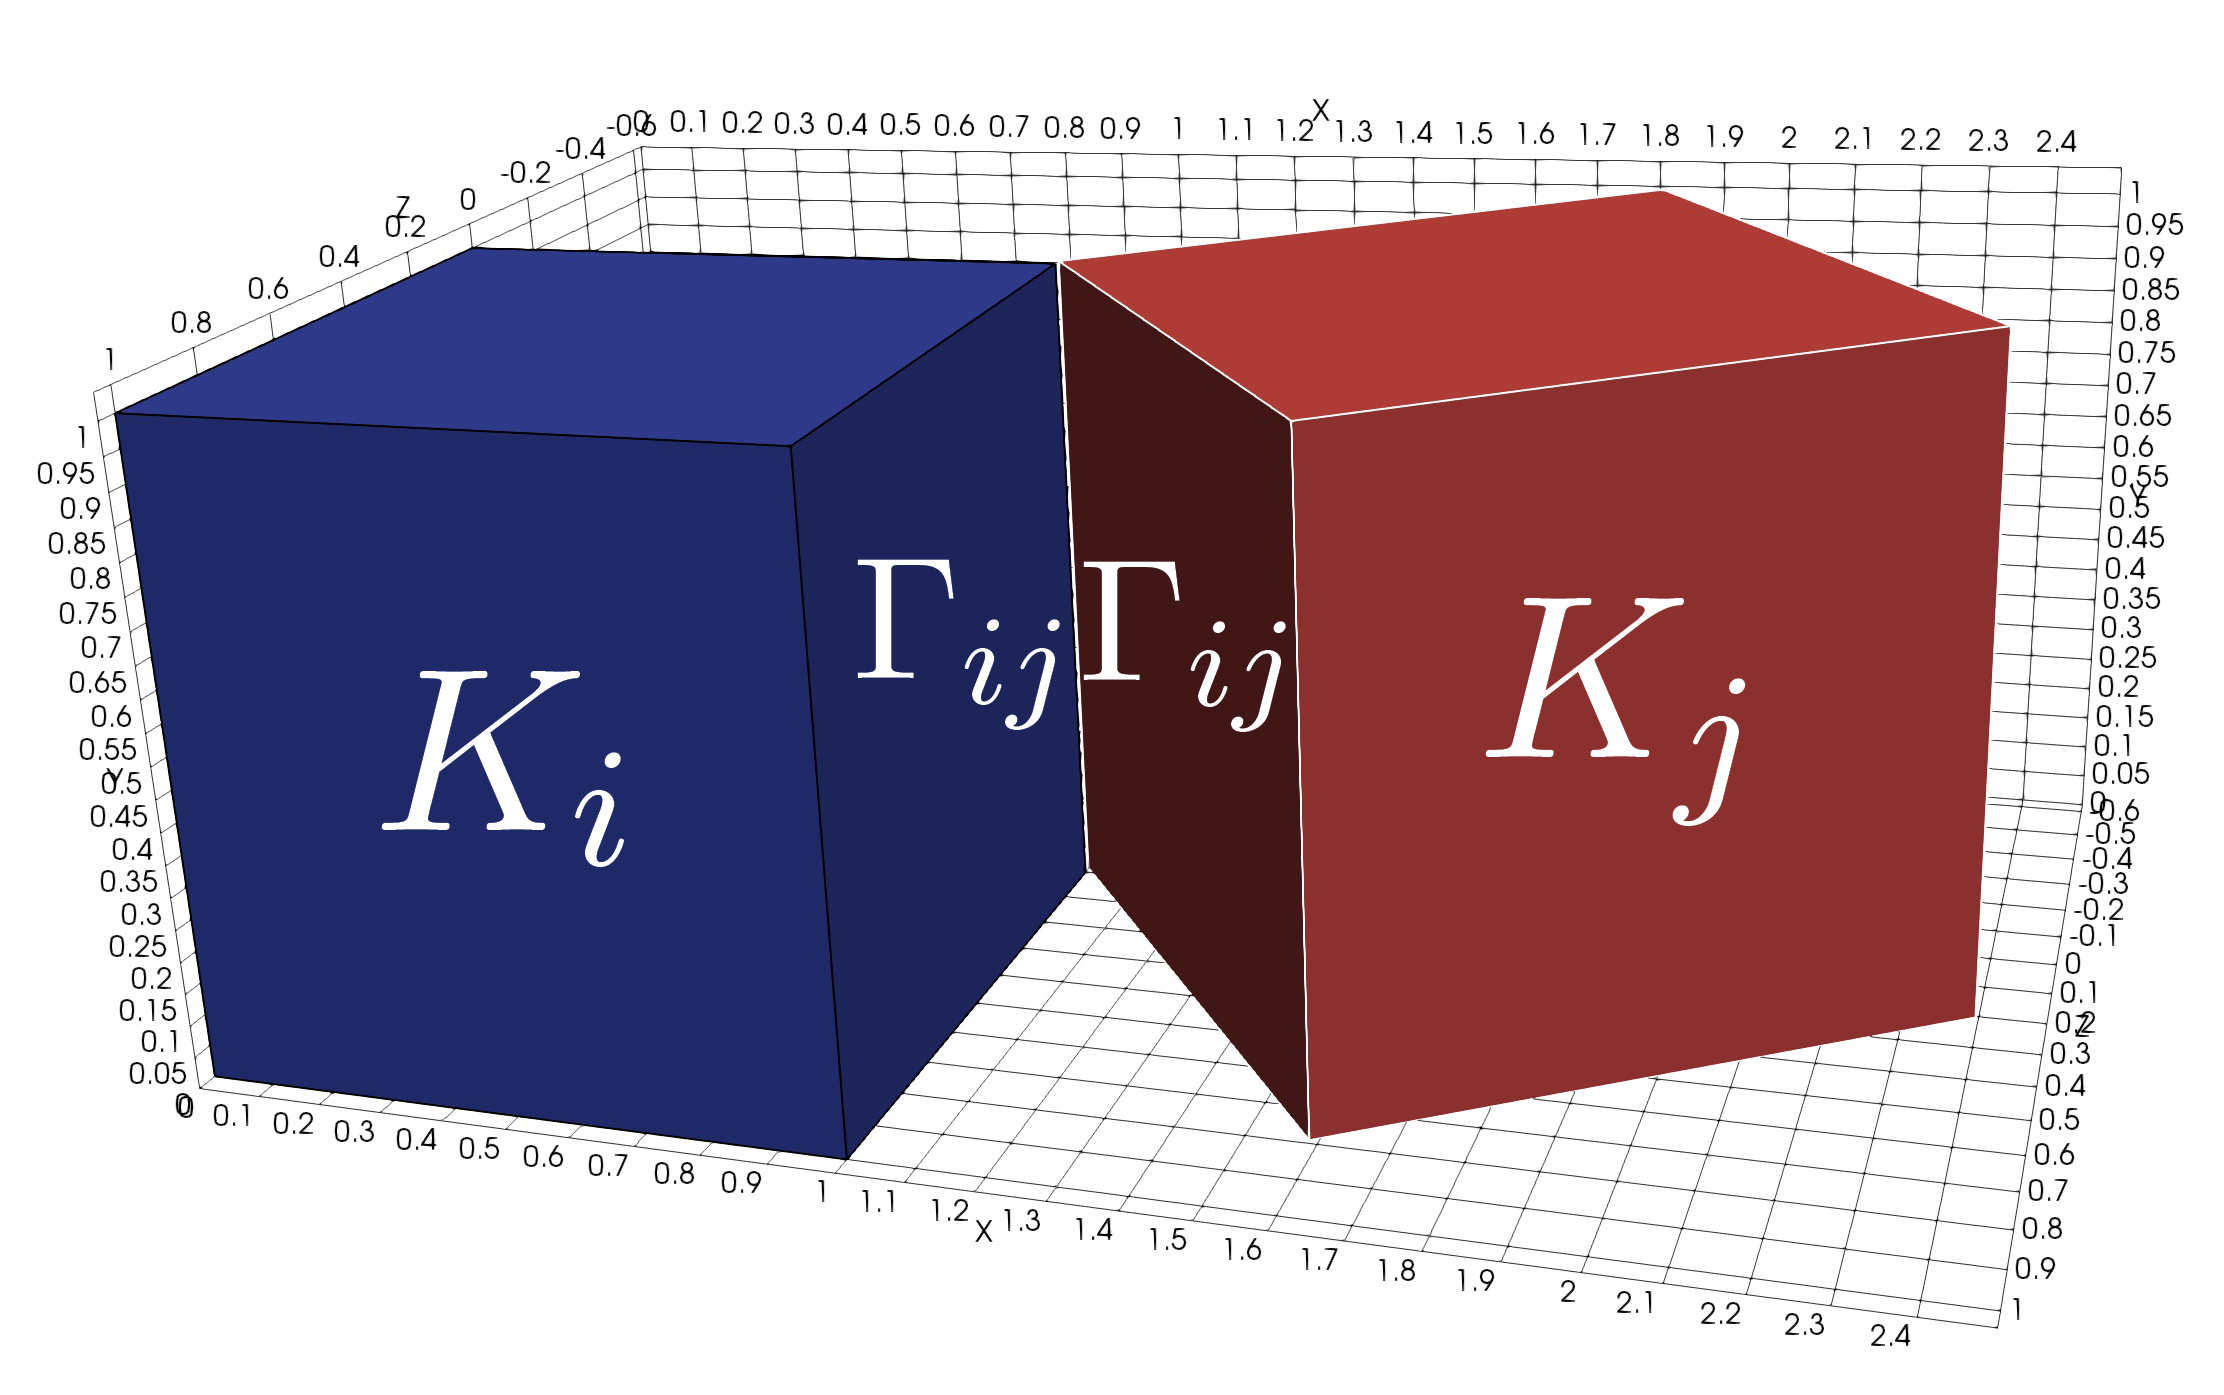
\includegraphics[width=0.5\textwidth]{img/mesh/neighborsSepK.jpg}
			\vspace{-5mm}
		\caption{Neighbor elements $K_i, K_j$ in the mesh (above), transformed in order to view $\Gamma_{ij}$ (below).}
		\label{figure:simpleNeighbors}
		\end{center}
	\end{figure}\vspace{-5mm}
	
If however, the two neighboring elements are not of the same size, situation gets more complicated. Note that for this work, the level of uniform refinement of the hexahedron $K_i$ must differ from the level of uniform refinement of any neighboring element $K_j$ with which it shares a common face $\Gamma_{ij}$ at most by one. This means that the situation when neighboring elements are not of the same side looks always as in \Cref{figure:worseNeighbors}, but $K_i$ can be on either side of $\Gamma_{ij}$ as indicated in \Cref{figure:worseNeighbors}. Note that the edge on the whole side of element $K_i$ is not physically stored anymore (at least not for assembling purposes).

\begin{figure}[H]
		\begin{center}
			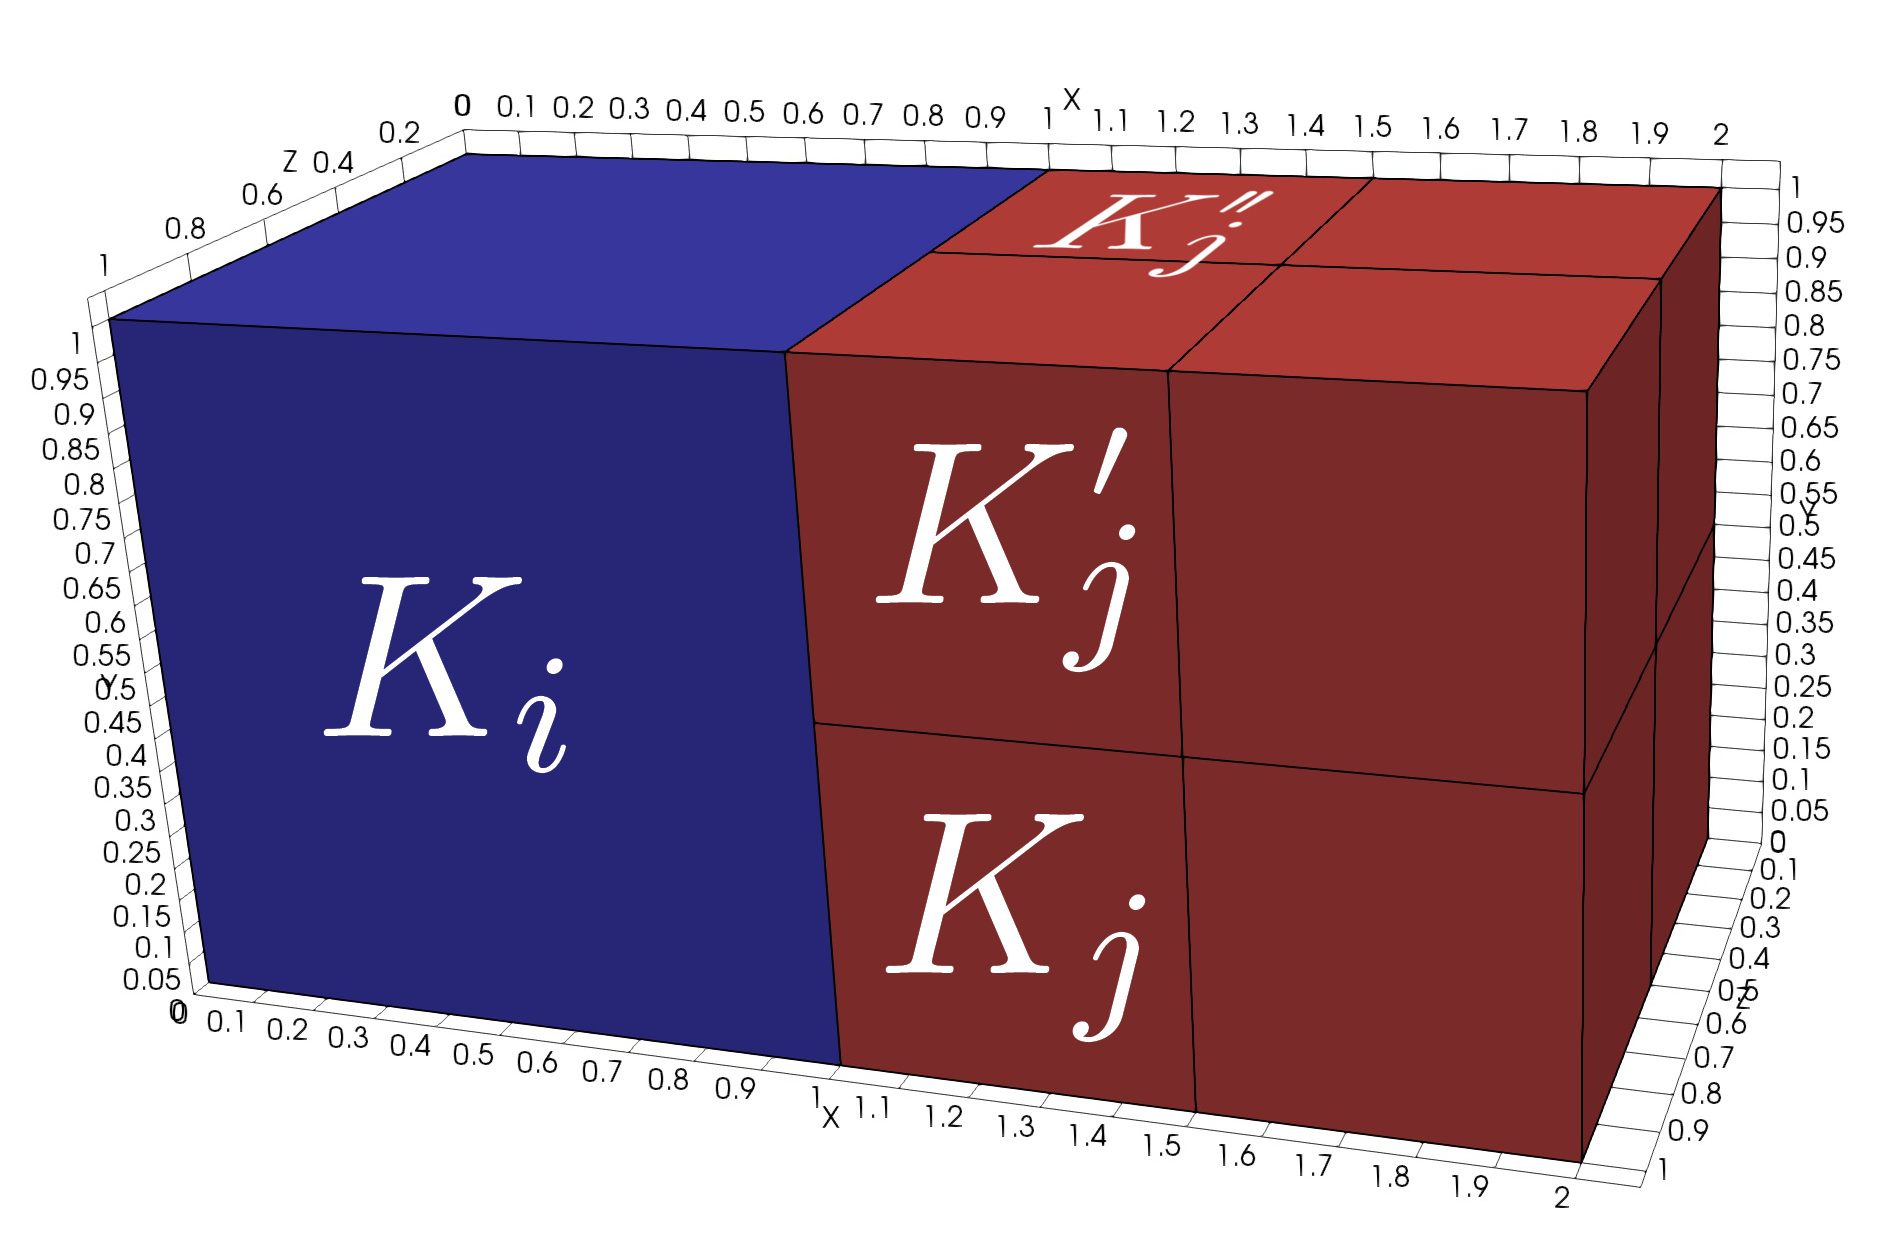
\includegraphics[width=0.5\textwidth]{img/mesh/neighborsOneLargerK.jpg}
			\vspace{3mm}
			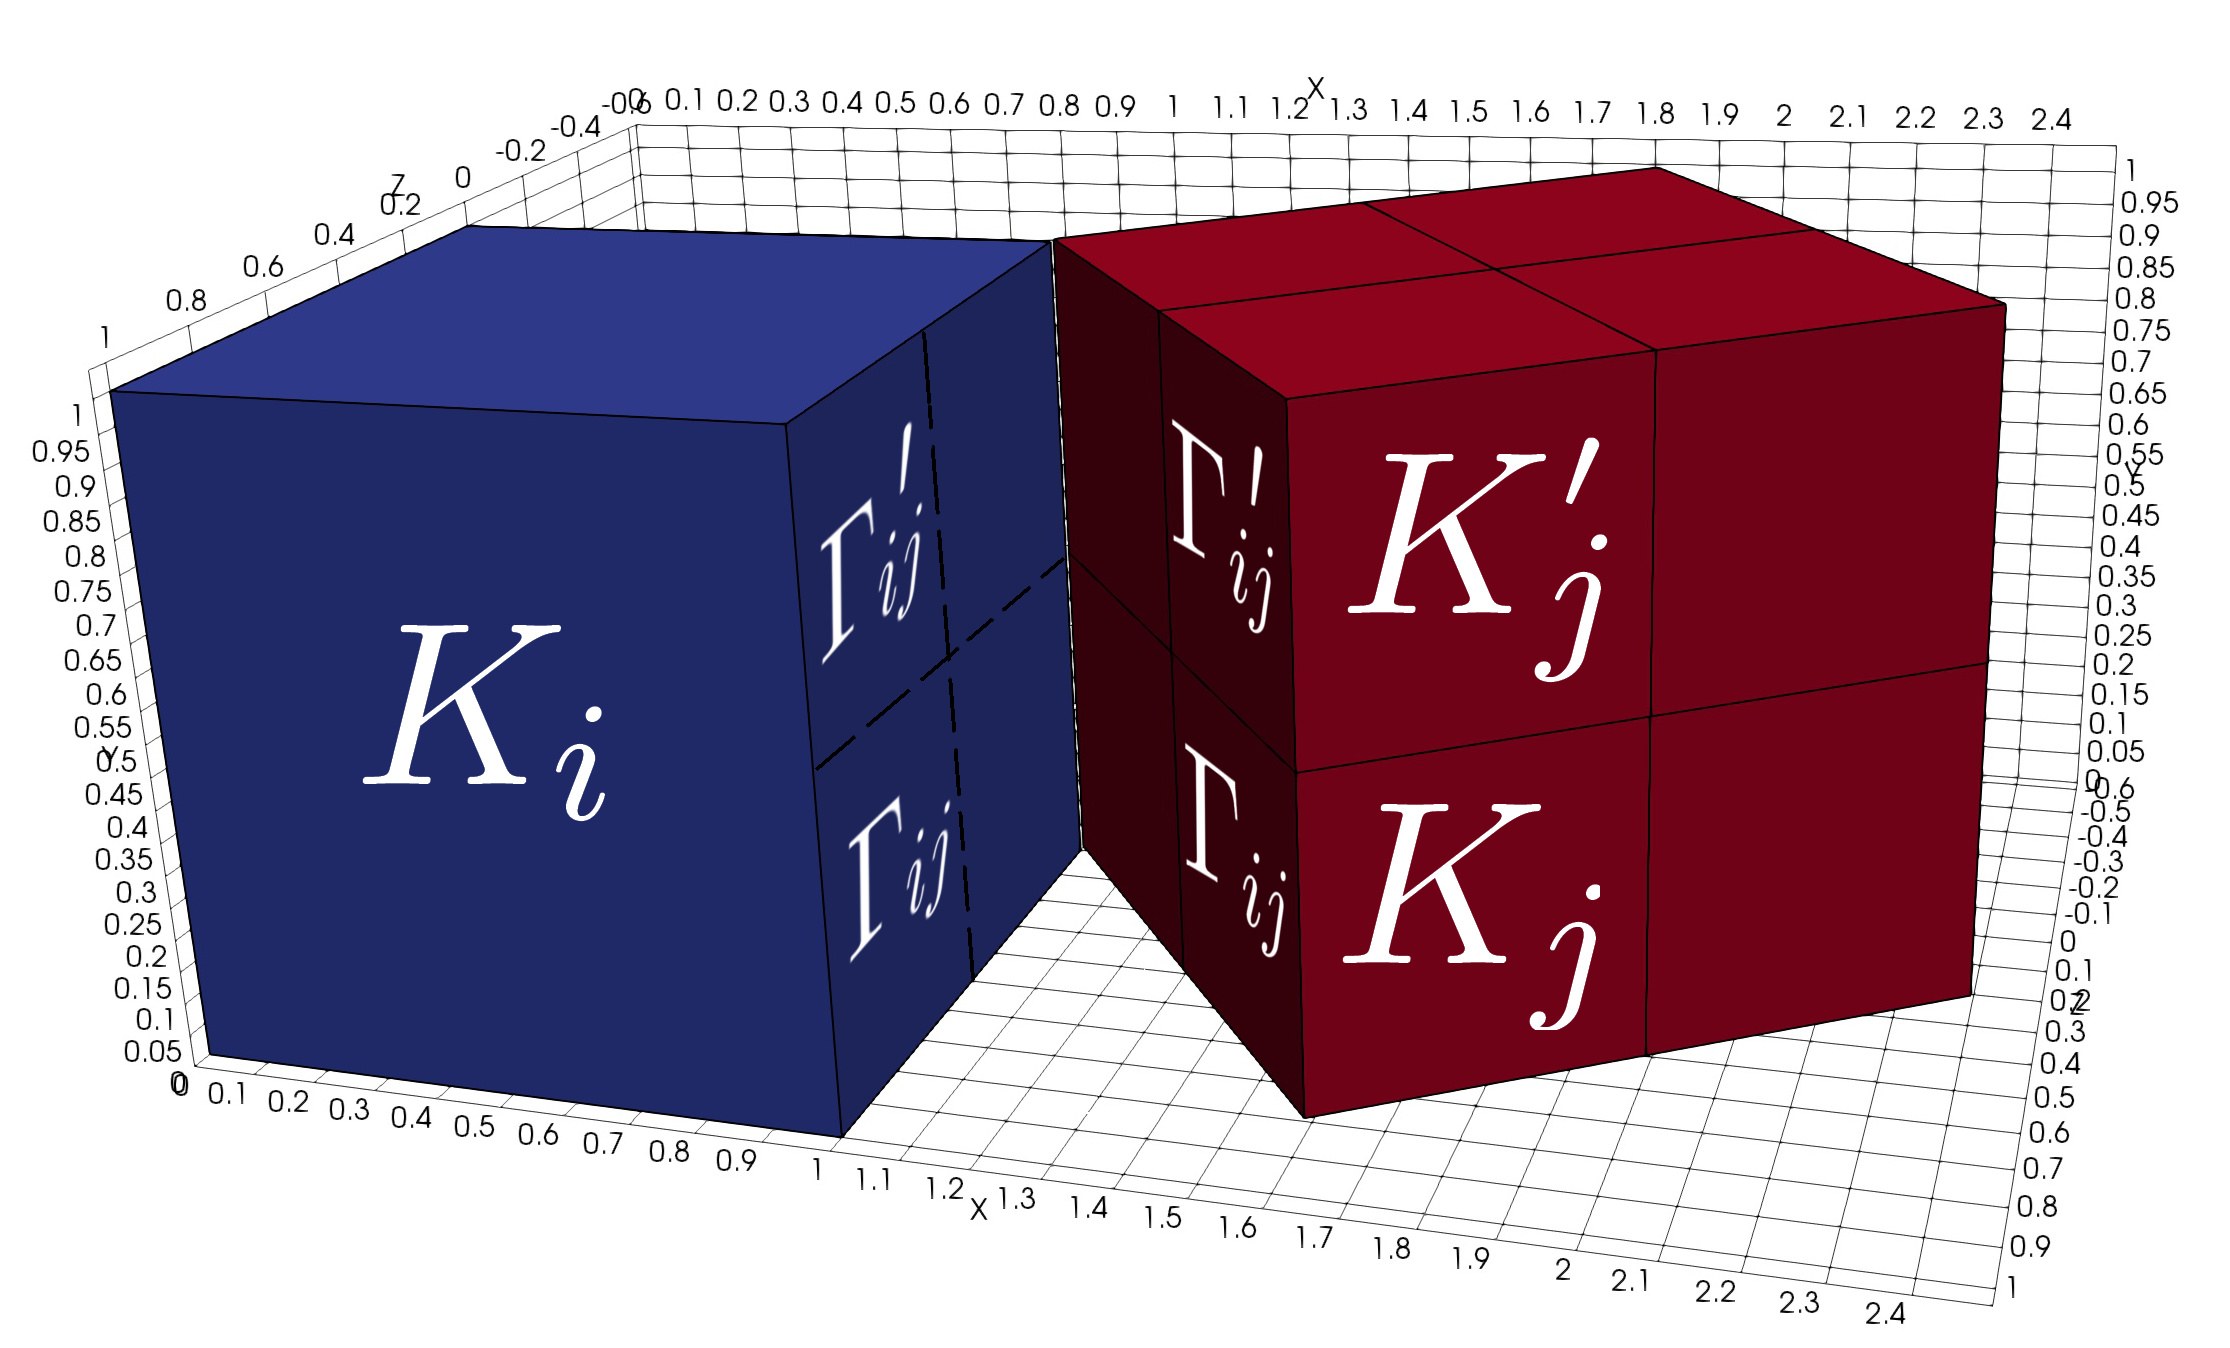
\includegraphics[width=0.5\textwidth]{img/mesh/neighborsOneLargerSepK.jpg}
			\vspace{-5mm}
		\caption{Neighbor elements $K_i, K_j, K_j^{'}, ...$ in the mesh (above), transformed in order to view $\Gamma_{ij}, \Gamma_{i{j^{'}}}$ (below).}
		\label{figure:worseNeighbors}
		\end{center}
	\end{figure}\vspace{-5mm}

\subsection{Periodic boundary conditions}
\label{amrPer}
Handling with periodic boundary conditions with AMR is primarily difficult because of implications for mesh partitioning - additional ghost cells need to be added to cells on boundaries with the periodic condition - in order to perform steps 1 and 2 in \Cref{algorithm:numFluxSimple}. See \Cref{figure:ghostPer}, and compare to \Cref{figure:ghost}.

\paragraph{}
The setup here is the same one used in \Cref{section:ditributedTria}, showing ghost elements as in \Cref{figure:ghost}, but periodic boundary conditions were added to the left-right and top-bottom boundary part pairs. And the necessary elements were thusly added to ghost elements set for each affected processor (processor having any elements on the periodic boundaries).

\begin{figure}[H]
		\begin{center}
			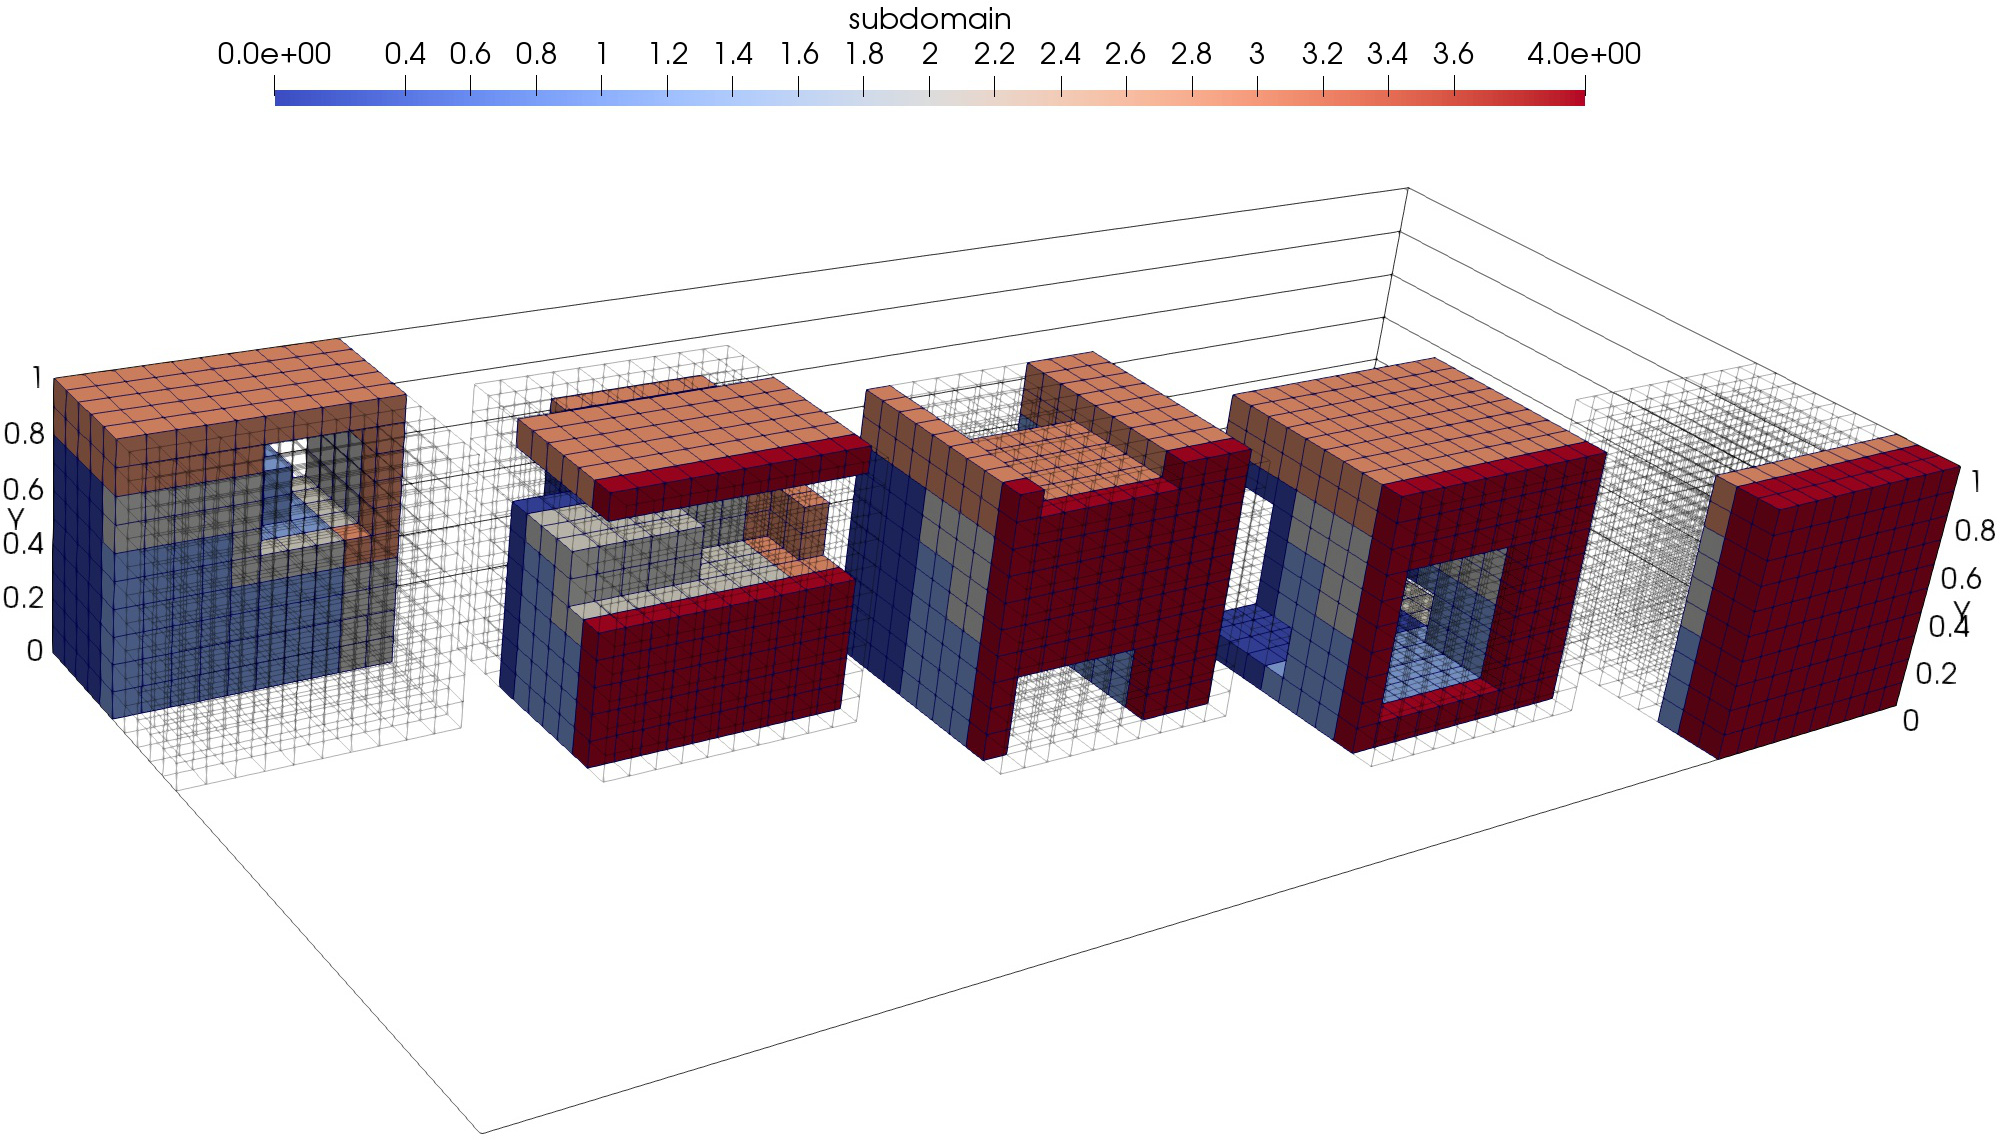
\includegraphics[width=0.78\textwidth]{img/mesh/cube-periodic,ghost.jpg}
			\vspace{-2mm}
		\caption{Processor-owned elements (0..4 left to right), with color-coded ghost elements from other processors. Ghost cells that have to be present here are dictated by fluxes - both across internal edges, and across periodic boundaries.}
		\label{figure:ghostPer}
		\end{center}
	\end{figure}\vspace{-5mm}

\subsection{Relationship with slope limiters}
As a key step in the slope limiting algorithm \Cref{algorithm:limiter} is forming the set of all elements $K_{\bfv} = \left\{K^{'}\in T\ |\ \bfv \text{ is a vertex of } K\right\}$ for a particular vertex $\bfv$, and as this step tends to be rather expensive for distributed triangulations (which have different topology than vertex-based), caching of the already obtained mappings between the vertex $\bfv$ and the set $K_{\bfv}$ is employed. Of course with every mesh refinement, a lot of these cached values need to be forgotten.
\paragraph{}
In reality, after each mesh refinement step, there follows a step of redistributing the mesh (to have roughly equal number of elements owned by each processors - that is to avoid bottlenecks where one processors would do a significant portion of all processing and other processors would idly wait for it to finish assembling). This is illustrated in \Crefrange{figure:blastOldMyAdapt1}{figure:blastOldMyAdapt6}.
\paragraph{}
From this it follows, that carefully computing which entries in such a cache must be forgotten and which not would be very tedious and complex - that is why, for pragmatic reasons, after each refinement step, the entire cache is flushed. But in order not to suffer from slope limiting being a costly operation, the mesh refinement is performed only in every $n$-th time step. Another reason to do so is that with the unchanged mesh, the algebraic solver can keep the once computed matrix structures and data alike, which again saves computational time.